\documentclass[aspectratio=169]{beamer}

\usepackage[T1]{fontenc}
\usepackage[utf8]{inputenc}
\usepackage[english]{babel}
\usepackage{geometry}
\geometry{paperwidth=210mm,paperheight=297mm}
\usepackage{lmodern}
\usepackage{tikz}
\usepackage{graphicx}
\usepackage{ragged2e} % for \justifying
\usetikzlibrary{positioning}

% Use Unipd as theme, with options:
% - pageofpages: define the separation symbol of the footer page of pages (e.g.: of, di, /, default: of)
% - logo: position another logo near the Unipd logo in the title page (e.g. department logo), passing the second logo path as option 
% Use the environment lastframe to add the endframe text
\usetheme[pageofpages=of]{Unipd}

\title{Vizualization Diary}
\subtitle{BDM-02 - Visual Analytics}
\author[Samuel Chapuis]{\and S.~Chapuis}

\date{\today}

% The next block of commands puts the table of contents at the beginning of each section and highlights the current section
\AtBeginSection[]
{
  \begin{frame}
    \frametitle{Table of Contents}
    \tableofcontents[currentsection]
  \end{frame}
}



\begin{document}

% Make the title page
\frame{\titlepage}

\begin{frame}{Week 1 — GitHub Contribution Calendar}
\small
\noindent
\begin{minipage}{0.4\textwidth}
  \centering
  \rotatebox{90}{\centering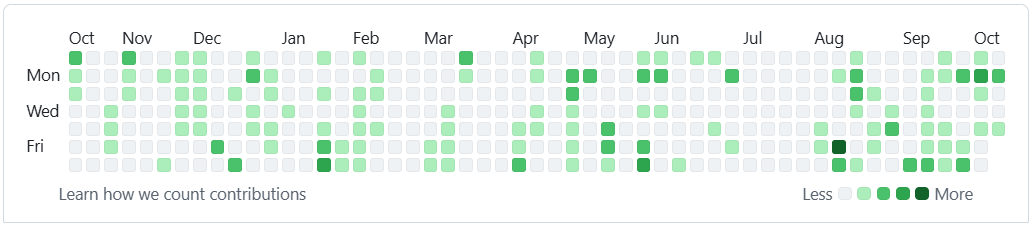
\includegraphics[height=0.5\linewidth]{image/git.png}}
  \hspace{20pt}
  \vrule width 0.5pt%
\end{minipage}
\begin{minipage}{0.5\textwidth}
  \centering
  \setlength{\parskip}{3mm}%
  \justifying
  \vspace{0pt} % Alignement en haut
  
  \textbf{How I found the visualization (and why I picked it)}\\
  I encountered this visualization directly on my GitHub profile dashboard. I chose it because it represents the trace of my own programming activity over the past year. It immediately attracted my attention because it condenses an entire year of work into a single, minimal grid of color.

  \vfill % Espace vertical flexible
  
  \textbf{What this visualization shows}\\
  The chart displays the number of GitHub contributions I made over the last twelve months (commits, pull requests, and issues). Each cell represents one day, colored from light to dark green according to the number of contributions. The layout follows a calendar logic, allowing users to see long-term rhythms of activity—periods of intense coding and quieter phases—at a glance.

  \vfill % Espace vertical flexible
  
  \textbf{Context}\\
  This visualization is automatically generated by GitHub to summarize user activity and encourage engagement. It is meant to highlight consistency, productivity, and growth within the open-source and developer community. The design is familiar to millions of programmers and serves both as a personal motivator and a public indicator of involvement.

  \vfill % Espace vertical flexible
  
  \textbf{Design choices}\\
  The simplicity of the grid and the sequential green color scale make it intuitive to read. However, the color contrast could be problematic for color-blind users, and the absence of numeric labels makes quantitative comparison difficult. The alignment by weeks and days supports quick temporal reasoning, though transitions between years can feel abrupt.

  \vfill % Espace vertical flexible
  
  \textbf{Improvements}\\
  For a more analytical audience, I would add interactive tooltips showing exact contribution counts and repository names. A second line chart could reveal trends in monthly or weekday averages. Finally, alternative palettes with higher contrast or color-blind-friendly schemes (e.g., blue–orange) would improve accessibility without losing aesthetic clarity.
  
  \vspace{0pt} % Alignement en bas
\end{minipage}
\end{frame}

%%%%%%%%%%%%%%%%%%%%%%%%%%%%%%%%%%%%
% EXEMPLE SLIDES
%%%%%%%%%%%%%%%%%%%%%%%%%%%%%%%%%%%%

% \section{First section}

%     \begin{frame}{First section}
%         In this slide, some important text will be
%         \alert{highlighted} because it's important.
%         Here an ordered list:
%         \begin{enumerate}
%             \item First item
%             \item Second item
%         \end{enumerate}
%         Here an unordered list: 
%         \begin{itemize}
%             \item One item
%             \item Another item
%         \end{itemize}
%     \end{frame}
    
% \section{Second section}

%     \begin{frame}{Second section}
%         \begin{block}{Block}
%             Sample text in a normal block
%         \end{block}
   
%         \begin{alertblock}{Alert block}
%             Sample text in an alert block
%         \end{alertblock}    
        
%          \begin{example}
%             Sample text for an example
%         \end{example}
%     \end{frame}

    
%     \begin{emptyframe}
%         Thank you!
%     \end{emptyframe}

%     \appendix

%     \begin{frame}{Backup slide}
%         Some additional content
%     \end{frame}
    
\end{document}